\documentclass[uplatex,dvipdfmx,a4j,12pt]{jsarticle}

\usepackage[utf8]{inputenc}
\usepackage{graphicx}
\usepackage{amsmath}
\usepackage{comment}
\usepackage{color}
\usepackage{url}
\usepackage{siunitx}
\usepackage[version=4]{mhchem}
\usepackage{paralist}
\usepackage{longtable}
\usepackage{multirow}
\usepackage[dvipdfmx]{hyperref}
\usepackage{pxjahyper}
\usepackage{subcaption}
\usepackage{here}
% \usepackage{makecell} % Add makecell package

\usepackage{enumitem}
\setlist[description]{parsep=5pt}
\setlist[enumerate]{parsep=5pt}

% コマンド定義
\newcommand{\divergence}{\mathrm{div}\,}  %ダイバージェンス
\newcommand{\grad}{\mathrm{grad}\,}  %グラディエント
\newcommand{\rot}{\mathrm{rot}\,}  %ローテーション
\newcommand{\diff}{\mathrm{d}} % 微分
\newcommand{\e}{\mathbf{e}} % 単位ベクトル


% 半角文字のパーセント、より右側は、コメントとして扱われます。

% タイトルページの内容をここで記述します。
\title{
  物理学実験IIレポート\\    % \\ は、強制的に改行するコマンドです。
  課題5 「電磁波の伝搬特性」
  }
\author{
  実験回: 第1回 \\
  氏名: 佐藤空馬\\
  実験者番号:28
  \\
  共同実験者:髙田和毅,福冨葵
  }
\date{
  実験日:2025年 4月 10日~ 5月 7日 \\
  提出日:2025年 5月 14日}  % 実験日と、提出日を記入して下さい

% ここから本文が始まります。
\begin{document}

% 上で設定したタイトルページの情報は、\maketitle があって始めて、コンパイル後に表示されます。
\maketitle

% レポートのフィードバックのコメントを希望しない場合には、
% 48行目から55行目までをコメントアウト(行頭に%を入れる)。
% コメントを希望する場合は、何について聞きたいかを具体的に書いて下さい。

% 縦方向の空白を挿入するコマンドです。em は行の高さ分、を意味する単位です。
% \vspace{2em}
% \begin{center}
%     \begin{minipage}{0.5\linewidth}
%         レポートのコメントを希望します。

%         具体的には、○○について評価を下さい。
%     \end{minipage}
% \end{center}

\vspace{5em}  


% 概要は論文・レポート全体を一つの段落にまとめたものです。
% 物理の分野では、概要では段落分けをしません。
%
\begin{abstract}
    % \textcolor{red}{このテンプレートにある指示文章は全て削除し、自分で書いた文章に差し替えること。残っていた場合は読みやすさを損ねるため減点とする。}
    % (概要ではレポートの概要を簡潔に記述せよ。例えば、以下のようなものである。)
    % ○○の目的のために、■■の実験を行った。
    % その結果△△であることが確かめられた。
  本実験では,高周波信号を取り扱う上で重要となるインピーダンスおよび電磁波の波動性について調べることを目的に,
  インピーダンス整合・不整合時の反射率,透過率の測定実験やアンテナの特性を調べる実験を行った.
  また,関連して高周波信号の検出を行う際によく用いられるヘテロダイン検波について,実際にローパスフィルタを作成して実験を行った.
  その結果,インピーダンスの整合時には反射が見られないことや,周波数に応じたインピーダンスの変化により反射率や透過率が変化すること,
  アンテナの距離・角度・周波数依存性などが確かめられた.
  また,ローパスフィルタを用いて混合した信号から信号を取り出せることが確認された.
\end{abstract}

% 強制的に改ページを行う
\newpage


\section{目的}
% この実験のねらいが何であるかを、教科書の$\S2$を参考に簡潔にまとめる。
高周波回路は現代の通信技術において重要な役割を果たすだけでなく, より高精度な実験・測定を行うための基礎技術でもある.
本実験では, 高周波領域で現れる電磁波の波動性に着目してその伝播特性を調べると共に, 素子のインピーダンスやそれに起因する信号の反射を調べることを目的とする.

\section{原理}
% この実験に関連する原理を、教科書の$\S2$を参考に簡潔に記述する。
\subsection{電磁波}
電磁波は、電場と磁場が互いに直交しながら進行する波動である.

Maxwellの方程式から, 真空中の電磁波に対する波動方程式は次のように表される:
\begin{equation}
    \nabla^2 \mathbf{E} - \frac{1}{c^2} \frac{\partial^2 \mathbf{E}}{\partial t^2} = 0
\end{equation}
ここで、$\mathbf{E}$は電場ベクトル, $c = 1/\sqrt{\epsilon\varepsilon}$は光速である.
したがって, $x$方向に進行する電磁波は次のように表される:
\begin{equation}
    \mathbf{E}(x,t) = \mathbf{E_0} \exp{[i(\omega t - kx)]}
\end{equation}
ここで、$\mathbf{E_0}$は電場ベクトルの振幅, $k$は波数, $\omega$は角周波数である.
磁場の波 (磁波) についても同様の式が成り立つ.

より一般の誘電率$\varepsilon$と透磁率$\mu$を持つ媒質中での伝播を考えると, 電磁波は次式で表される:
\begin{equation}
  \mathbf{E}_x = \mathbf{E_0}\exp{(-\alpha z)} \exp{[i(\omega t - \beta z)]}
\end{equation}
ここで, 
\begin{gather}
  \alpha = \sqrt{\frac{\omega^2 \mu \varepsilon}{2} \left(\sqrt{1 + \frac{\sigma^2}{\omega^2 \varepsilon^2}} - 1\right)}, \\
  \beta = \sqrt{\frac{\omega^2 \mu \varepsilon}{2} \left(\sqrt{1 + \frac{\sigma^2}{\omega^2 \varepsilon^2}} + 1\right)},
\end{gather}
であり, $\sigma$は導電率である.

一般に$\sigma$は十分大きいと仮定できるので, $\alpha$は次のように近似できる:
\begin{equation}
  \alpha \approx \sqrt{\frac{\omega^2 \mu \varepsilon}{2} \frac{\sigma}{\omega \varepsilon}} = \sqrt{\frac{\omega \mu}{2 \rho}}
\end{equation}
ここで, $\rho = 1 / \sigma$は導体の抵抗率である.
したがって, 電磁波が媒質に侵入できる深さ (表皮深さ) $\delta$は次のように表される:
\begin{equation}
  \delta = \frac{1}{\alpha} = \sqrt{\frac{2 \rho}{\omega \mu}}.
  \label{eq:skin_depth}
\end{equation}

\enskip

次に, 伝送経路中を伝播する電磁波について述べる.
ここでは平行導線 (レッヘル線) や同軸ケーブルといった, 比較的簡単で等価回路を用いて議論できる系について考える.

レッヘル線を模した平行導線とその等価回路の模式図を図\ref{fig:lecher_line}に示す.
\begin{figure}[h]
    \centering
    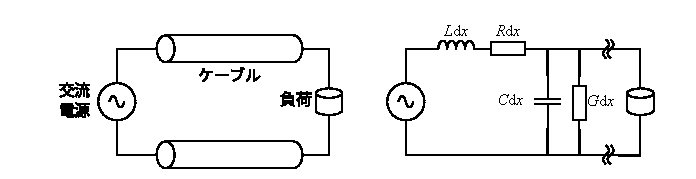
\includegraphics[width=0.9\linewidth]{img/lecher_line.pdf}
    \caption{平行導線 (左) とその等価回路 (右).}
    \label{fig:lecher_line}
\end{figure}

等価回路に示したように, 平行導線には単位長さあたりの抵抗$R$のほかに, 単位長さあたりのインダクタンス$L$, 
2つの導線間の静電容量$C$, コンダクタンス$G$が存在する.
このとき, 直列インピーダンス$Z$は$Z = R + i\omega L$, 並アドミニスタンス$Y$は$Y = G + i\omega C$と表される.
微小長さ$\diff z$間で生じる電位差$\diff V$と, 電流の変化$\diff I$は次のように表される:
\begin{equation}
  \frac{\diff V}{\diff x} = - Z I, \quad \frac{\diff I}{\diff x} = - Y V.
\end{equation}
ここから, 導線の特性インピーダンス$Z_0$を求めると,
\begin{equation}
  Z_0 = \frac{V}{I} = \sqrt{\frac{Z}{Y}} 
\end{equation}
一般に高周波伝達線路での損失は小さいことから, $R \ll 1$, $G \ll 1$と仮定できる.
したがって, $Z_0$は次のように近似できる:
\begin{equation}
  Z_0 \approx \sqrt{\frac{i\omega L}{i\omega C}} = \sqrt{\frac{L}{C}}.
\end{equation}
また, このとき伝達経路中の伝送速度として,
\begin{equation}
  v = \frac{1}{\sqrt{LC}}
\end{equation}
が成り立つ.

\enskip

同軸ケーブルにおいては, 単位長さあたりのインダクタンス$L$, 単位長さあたりの静電容量$C$は次のように表される:
\begin{equation}
  L = \frac{\mu_0}{2\pi} \ln\left(D/d\right), \quad C = \frac{2\pi\varepsilon_r \varepsilon_0}{\ln\left(D/d\right) }
\end{equation}
ここで, $D$は同軸ケーブルの外径, $d$は内径, $\varepsilon_r$は外部導体と中心導体の間の比誘電率である.

したがって, 同軸ケーブル中の伝送速度は次のように表される:
\begin{equation}
  v = \frac{1}{\sqrt{LC}} = \frac{c}{\sqrt{\varepsilon}} < c \label{eq:velocity_cable}
\end{equation}

\enskip

また, 電磁波の特徴的な性質として, 異なる媒質へ入射したときの反射と透過がある.

媒質1から媒質2へ入射したとき, 反射率$\Gamma$と透過率$T$は次のように表される:
\begin{align}
  \Gamma &= \frac{Z_2 - Z_1}{Z_2 + Z_1}, \label{eq:reflection}\\
  T &= \frac{2Z_1}{Z_2 + Z_1}
\end{align}
ここで, $Z_1$は媒質1のインピーダンス, $Z_2$は媒質2のインピーダンスである.
このことから,2媒質のインピーダンスが異なるときには,必ず反射が生じることが分かる.

この結果として,信号線の末端に負荷を接続した場合においても,負荷のインピーダンスが信号線のインピーダンスと異なるときには反射が生じる.
入力側のインピーダンスを$Z_0$,負荷のインピーダンスを$Z_L$とするとき,反射係数$\Gamma$は次のように式\eqref{eq:reflection}と同じ表式で表される:
\begin{equation}
  \Gamma = \frac{Z_L - Z_0}{Z_L + Z_0} \label{eq:reflection_2}
\end{equation}

抵抗器のインピーダンスは抵抗値と等しいことから,末端を開放した際には$Z_L = \infty$,$\Gamma = 1$,短絡した際には$Z_L = 0$,$\Gamma = -1$となる.
また,負荷のインピーダンスが信号線のインピーダンスと等しい場合には,$\Gamma = 0$となり,反射は生じない.

負荷としてコイルやコンデンサを接続した場合には,そのインピーダンスは周波数に依存した複素数となることから,周波数に応じて位相差$\sigma$が変化する.
式\eqref{eq:reflection_2}から, 
\begin{alignat}{4}
  &\text{コイル}\quad & Z_L &= i\omega L, & |\Gamma| &= 1, & \delta &= 2\arctan\left(\frac{ Z_0}{ \omega L}\right) \label{eq:coil_phase}\\
  &\text{コンデンサ}\quad & Z_L &= \frac{1}{i\omega C},\, & |\Gamma| &= 1,\, & \delta &= -2\arctan\left({Z_0\omega C}\right) \label{eq:condenser_phase}
\end{alignat}
となることわかる.

次に,$Z_L$の負荷が線路の途中に接続されている場合について考える.
この場合には,反射率は次のように表される:
\begin{equation}
  \Gamma = -\frac{Z_0}{2Z_L + Z_0}
  \label{eq:reflection_3}
\end{equation}
また,負荷の先の線路への透過率については,
\begin{equation}
  T = \frac{2Z_L}{2Z_L + Z_0}
  \label{eq:transmission}
\end{equation}
となる.すなわち,負荷がない場合$Z_L = \infty$では 反射率$\Gamma =  0$, 透過率$T = 1$となるが,負荷がある場合には透過率は1よりも小さくなることがわかる.


\subsection{共振回路}
回路の大きさが波長に比べて十分小さい集中定数回路においては,コイルやコンデンサを組み合わせることで共振回路を構成することができる.

$LRC$直列回路においては,回路のインピーダンス$Z$が,
\begin{equation}
  Z = R + i\omega L - \frac{i}{\omega C}, |Z| = \sqrt{R^2 + \left(\omega L - \frac{1}{\omega C}\right)^2}
\end{equation}
であることから,$\omega_0 L = 1/\omega_0 C$のとき,$|Z|$が最小となり,系に流れる電流は最大となる.
この現象を共振と呼び,その周波数 (共振周波数) を$f_0$とすると,
\begin{equation}
  f_0 = \frac{\omega_0}{2\pi} = \frac{1}{2\pi\sqrt{LC}}.\label{eq:resonance_frequency}
\end{equation}
となる.

回路の大きさが波長に比べて無視できないほど大きい場合には,分布定数回路と呼ばれる回路を考えることができる.

例えば,長さ$d$の伝送線路の先に反射率$\Gamma$の負荷を接続した場合,距離$d$間での位相変化を無視できないことから,入力側からみた回路の特性インピーダンスは,
\begin{equation}
  Z_d = \frac{1+\Gamma \exp{(-2ikd)}}{1-\Gamma \exp{(-2ikd)}}Z_0
\end{equation}
と表され,$\Gamma$が正の実数であるとき,$|Z_d|$が最小となるのは,
\begin{equation}
  d = (2n + 1)\frac{\lambda}{4}, \quad (n = 0, 1, 2, \cdots)\label{eq:resonance_length}
\end{equation}
となるときである.
これは自由端-固定端の共鳴条件と同じである.

\subsection{ヘテロダイン検波}
高周波 (搬送波) を別の周波数の信号と混合することで,情報を伝達することができる.
混合の手法には,搬送波の振幅を変化させる振幅変調 (AM),搬送波の周波数や位相を変化させる周波数変調 (FM)や位相変調がある

ヘテロダイン検波とは,搬送波と信号を混合することで,信号の周波数を変化させる手法である.
本実験ではダブルバランスドミキサ (DBM) を用いて,周波数混合を行った.
周波数$f$, 位相$\delta$の高周波信号をDBMのRF端子へ入力し,LO端子には高周波信号と僅かに異なる周波数$f_L$の高精度局所信号を入力することで,IF端子には信号の積として,
\begin{align}
  E_\mathrm{IF} &\propto E_\mathrm{RF} E_\mathrm{LO} \nonumber \\
  &\propto \cos\left(2\pi f t + \delta\right) \cos\left(2\pi f_L t\right) \nonumber \\
  &\propto \cos\left(2\pi (f + f_L) t + \delta\right) + \cos\left(2\pi (f - f_L) t + \delta\right)
\end{align}
なる,高周波成分$f + f_L$と低周波成分$f - f_L$の混ざった信号が得られる.
この信号をローパスフィルタで低周波成分 (中間周波数) のみを取り出すことで,高周波信号の振幅に比例し, 位相情報を含む信号 (ダウンコンバート信号)を得ることができる.

\subsection{ダイポールアンテナ}
電流が時間的に変化する導体の周りには, 電場と磁場が発生する.
また逆に, 電場と磁場の時間変化によって電流が生じる.
これを利用して, 電磁波を放射・受信する素子をアンテナと呼ぶ.
ここでは, 図\ref{fig:dipole_antenna}に示すようなダイポールアンテナについて考える.
\begin{figure}[h]
    \centering
    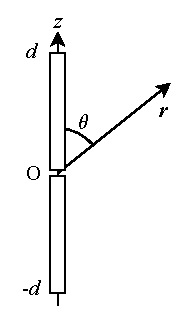
\includegraphics[width=0.2\linewidth]{img/dipole_antenna.pdf}
    \caption{ダイポールアンテナの模式図.}
    \label{fig:dipole_antenna}
\end{figure}

ダイポールアンテナの電流分布は次のように表される:
\begin{equation}
    I(x) = I_0 \left(1 - \frac{|z|}{d}\right)\sin\left(\omega t\right)
\end{equation}
ここで, $\omega$は印加する交流電源の角周波数であり,アンテナ上で電流の位相は等しいと仮定している.
このとき, 保存の式から電荷密度について次のように表される:
\begin{equation}
  \frac{\partial \rho}{\partial t}  = - \frac{\partial I}{\partial z} = \pm \frac{I_0}{d}\sin\left(\omega t\right)
\end{equation}
したがって, 
\begin{equation}
  \rho = \mp \frac{I_0}{\omega d}\cos\left(\omega t\right)
\end{equation}

このとき, 双極子モーメント$\mathbf{p}$は次のように表される:
\begin{equation}
  \mathbf{p} = \int \rho \mathbf{r} dV = \mp \frac{I_0}{\omega d}\int \cos\left(\omega t\right) \mathbf{r} dV
  = -\frac{I_0 d}{\omega}\cos\left(\omega t\right) \mathbf{e}_\mathrm{z}.
\end{equation}

ここで, 双極子から十分離れた点$\mathbf{r}$でのポインティングベクトル$\mathbf{S}$は次のように表される:
\begin{equation}
  \mathbf{S} = \frac{1}{\mu_0}\left(\mathbf{E} \times \mathbf{H}\right) =
  \frac{\mu_0}{(4\pi)^2c} \frac{\ddot{p}(t)\sin^2\theta}{r^2}\mathbf{e}_\mathrm{r}
\end{equation}
ここで, $\theta$は位置$\mathbf{r}$と双極子$\mathbf{p}$のなす角度であり, $\mathbf{e}_\mathrm{r}$は位置ベクトルの単位ベクトルである.
したがって, 電磁波のエネルギー流束は次のように表される:
\begin{equation}
  \mathbf{S} = \frac{\mu_0}{(4\pi)^2c} \frac{\sin^2\theta}{r^2}(I_0 d \omega)^2 \cos^2\left(\omega t\right)\,\mathbf{e}_\mathrm{r}
\end{equation}
時間平均をとると,
\begin{equation}
  \langle \mathbf{S} \rangle = \frac{\mu_0}{(4\pi)^2c} \frac{\sin^2\theta}{r^2}(I_0 d \omega)^2 \frac{1}{2}\,\mathbf{e}_\mathrm{r}
\end{equation}
となる.

したがって, 距離$r$離れた点で受信するとき, 受信側で得られる電力$P$は次のように表される:
\begin{equation}
  P \propto |\langle \mathbf{S} \rangle| \propto \frac{\sin^2\theta}{r^2} \label{eq:power_received}
\end{equation}

\section{課題1: 高周波信号測定の基礎}
\subsection{オシロスコープによる測定}
\subsubsection{方法}
% 方法について簡潔に記述する。
% 必要に応じて回路図や実験装置の配置を挿入する。テキストに記載された図と等価な場合は、「テキスト図XXの回路を用いて...」のように引用してよい。
実験に用いた回路はテキスト図16 (p. 141) と同様であり, ファンクションジェネレータで発生させた信号をパワーディバイダによって分割し, 1 [m]の同軸ケーブルを介して, オシロスコープに接続させた.

このとき, まず初めにオシロスコープで測定された信号振幅からパワーディバイダが信号を均等に分割できていることを確かめた.
ただし, 測定のしやすさから, 以降断りのない限りは振幅としてPeak to Peak (PP) 値を用いる.

そのうえで, オシロスコープのCh.2の入力カップリングをDC 50 \si{\ohm}からDC 1M \si{\ohm}に変更し, Ch.1とCh.2の信号波形を比較した.
また, Ch.2に50 [\si{\ohm}] の貫通ターミネータを接続し, 信号波形の変化を観察した.

次に, Ch.2の入力カップリングをDC 50\si{\ohm}に戻した上で,ファンクションジェネレータの出力部分に6 dBの減衰器を接続し, Ch.1とCh.2の信号波形を比較するとともに, 信号の減衰を測定した.
さらに, Ch.2に接続する同軸ケーブルの長さを10 [m]に変更し, Ch.1とCh.2の信号の位相差 (立上りの時間差) を測定し, これによって信号の伝達速度を求めた.



\subsubsection{結果}
% 実験で得た結果を記す。
% 例えば、実験データの表、グラフなどを記載し、それらについて文章で説明する。
入力カップリング50\si{\ohm}においてCh.1とCh.2の信号波形を比較した結果のCh.1, Ch.2の信号振幅を表\ref{table:1-1-1}に示す.
\begin{table}[h]
    \centering
    \caption{オシロスコープのCh.1, Ch.2の信号振幅.}
    \label{table:1-1-1}
    \begin{tabular}{cc}
        \hline
        & 信号振幅 [mV]\\
        \hline\hline
        Ch.1 & 920  \\
        Ch.2 & 860  \\
        \hline
    \end{tabular}
\end{table}
Ch.1の信号振幅は920 [mV], Ch.2の信号振幅は860 [mV]であり, 2つの信号はほぼ同じ振幅であることがわかる.

次に, Ch.2の入力カップリングをDC 1M \si{\ohm}に変更した場合の信号波形を比較した結果のCh.1, Ch.2の信号振幅を表\ref{table:-1-1-2}に示す.
\begin{table}[h]
    \centering
    \caption{入力カップリングをDC 1M \si{\ohm}に設定したときのオシロスコープのCh.1, Ch.2の信号振幅.}
    \label{table:-1-1-2}
    \begin{tabular}{ccc}
        \hline
        & 信号振幅 [V] & 貫通ターミネータ接続後 [mV]\\ % Use \makecell for line break
        \hline\hline
        Ch.1 & 1.35 & 920 \\
        Ch.2 & 1.76 & 890\\
        \hline
    \end{tabular}
\end{table}
図に示したように, 入力カップリングをDC 1M \si{\ohm}に変更することで, 観測された信号振幅の増大が確認できた.
また図\ref{table:-1-1-2}に示すように, 貫通ターミネータを接続した場合の信号振幅はCh.1が920 [mV], Ch.2が890 [mV]であり, いずれも元の状態に戻ったことがわかる.

次に, Ch.2の入力カップリングをDC 50\si{\ohm}に戻した上で,ファンクションジェネレータの出力部分に6 dBの減衰器を接続し, Ch.1とCh.2の信号波形を比較した結果のCh.1, Ch.2の信号振幅を表\ref{table:1-1-3}に示す.
\begin{table}[h]
    \centering
    \caption{オシロスコープのCh.1, Ch.2の信号振幅.}
    \label{table:1-1-3}
    \begin{tabular}{ccc}
        \hline
        & 信号振幅 [mV]& 減衰率[dB]\\
        \hline\hline
        Ch.1 & 468 & 5.87\\
        Ch.2 & 437 & 5.88\\
        \hline
    \end{tabular}
\end{table}
Ch.1の信号振幅は468 [mV], Ch.2の信号振幅は437 [mV]であり, 最初の状態からの減衰率はdBで表すとそれぞれ5.87 [dB], 5.88 [dB]であった.
これは, 減衰器の減衰率が6 [dB]であることから, 減衰器の設計値とほぼ一致していることがわかる.

最後に, Ch.2に接続する同軸ケーブルの長さを10 [m]に変更し, Ch.1とCh.2の信号の位相差を測定した結果, $\Delta t = 45.6$ [ns]であった.
このとき, 信号中を伝達する電磁波の伝達速度$c_\mathrm{cable}$は,
\begin{equation}
  c_\mathrm{cable} = \frac{L}{\Delta t} = \frac{9\,\mathrm{[m]}}{45.6 \times 10^{-9}\,\mathrm{[s]}} \approx 2.0 \times 10^8 \mathrm{\,[m/s]}
\end{equation}

と求まる.







\subsubsection{考察}
% テキストに記載された考察事項に沿った考察を記入する。
% 上記に加えて、独自の視点での考察も記すことを推奨する。


原理の節の式\eqref{eq:velocity_cable} に示したように,誘電体中における光速は真空中の光速$c$よりも遅くなる.
式\eqref{eq:velocity_cable}を逆に解くことにより,測定された伝達速度$c_\mathrm{cable}$から同軸ケーブルの誘電率$\varepsilon_\mathrm{cable}$を求めることができる:
\begin{equation}
  \varepsilon_\mathrm{cable} = \left(\frac{c}{c_\mathrm{cable}}\right)^2 \approx \left(\frac{3.0 \times 10^8\,\mathrm{[m/s]}}{2.0 \times 10^8\,\mathrm{[m/s]}}\right)^2 \approx 2.3
\end{equation}
これは, 同軸ケーブルによく用いられる誘電体であるポリエチレンの誘電率$\varepsilon_\mathrm{PE} \approx 2.3$とよく一致していることが分かる.



\subsection{パワーメータによる測定}
\subsubsection{方法}
まず始めに,同軸ケーブルにおよる信号の減衰を測定するために,テキスト図17のように標準信号発生器からの信号をパワーディバイダで分割し,1 [m]と10 [m]の同軸ケーブルを介してパワーメータのA, B端子に接続した.
パワーメータでは,A端子の電力およびA, B端子の電力比を測定することができる.
標準信号発生器から出力 0 [dBm] の正弦波を発生させ,その周波数を変えることでA端子の信号電力とA, B端子の電力比の周波数依存性を測定した.

次に,テキスト図18のように1 [m] と10 [m] 同軸ケーブルを並列に接続することで信号の重ね合わせを行った.
このとき,先と同様に出力 0 [dBm] の正弦波を入力し,A端子で測定される電力とA, B端子の電力比の周波数依存性を測定した.

\subsubsection{結果}
まず始めに,同軸ケーブルによるい信号の減衰について測定した結果を次の図\ref{fig:1_1}および図\ref{fig:1_2}に示す.
\begin{figure}[H]
    \centering
    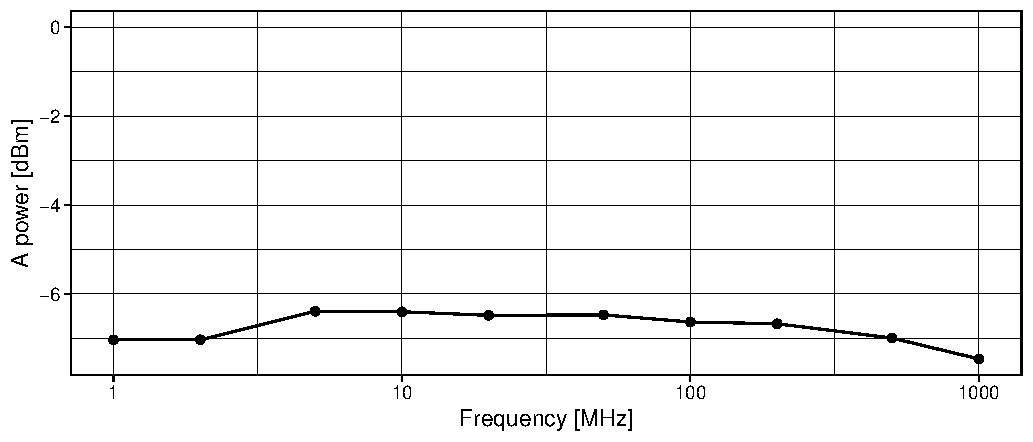
\includegraphics[width=0.9\linewidth]{data/1_1/power_vs_freq.pdf}
    \caption{Aの信号電力の周波数依存性.}
    \label{fig:1_1}
\end{figure}  

\begin{figure}[H]
  \centering
  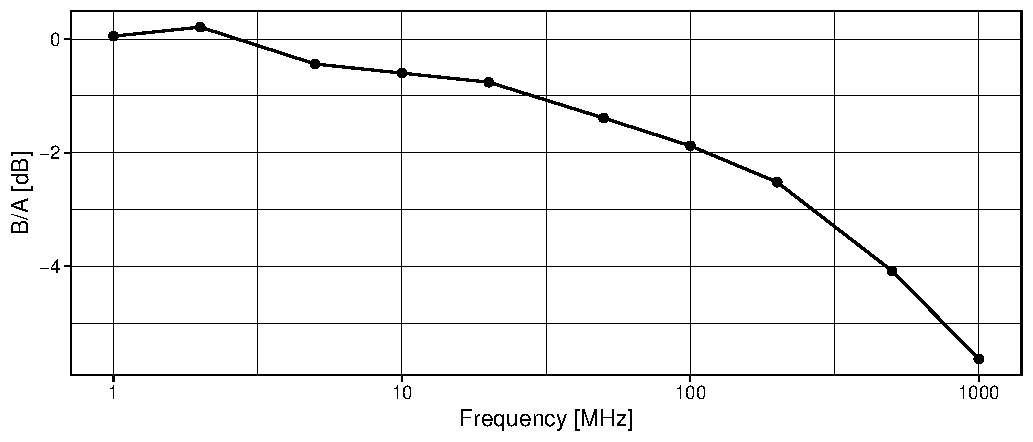
\includegraphics[width=\linewidth]{data/1_1/power_ratio_vs_freq.pdf}
  \caption{AとBの電力比の周波数依存性.}
  \label{fig:1_2}        
\end{figure}

また,図\ref{fig:1_2}から,単位長さ当たりの減衰率を求めた結果が,次の図\ref{fig:1_3}である.
\begin{figure}[H]
  \centering
  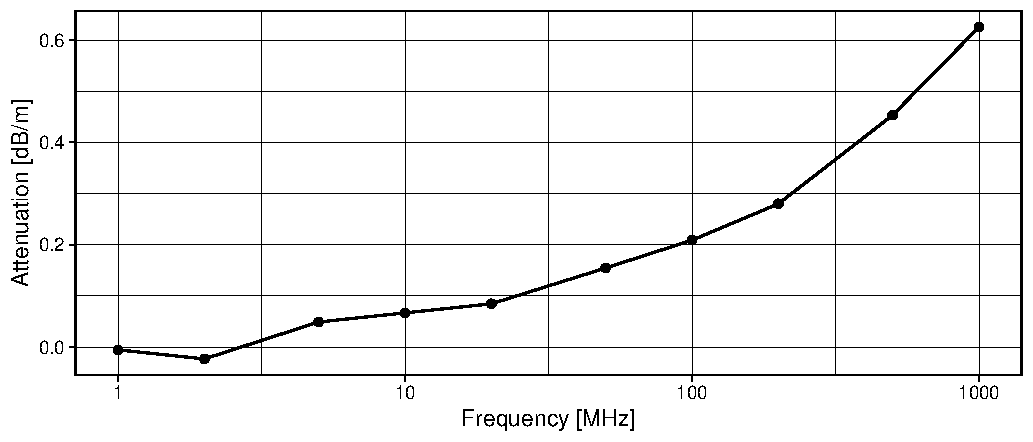
\includegraphics[width=\linewidth]{data/1_1/decay_ratio_vs_freq.pdf}
  \caption{同軸ケーブルの減衰率の周波数依存性.}
  \label{fig:1_3}
\end{figure}

高周波ほど,単位長さ当たりの減衰率が大きくなっていることが分かる.
一方で,A端子に入力される信号電力は,周波数によって変化しないことが分かった.


次に,同軸ケーブルを並列に接続することで信号の重ね合わせを行った結果を次の図\ref{fig:1_4}および図\ref{fig:1_5}に示す.
\begin{figure}[H]
  \centering
  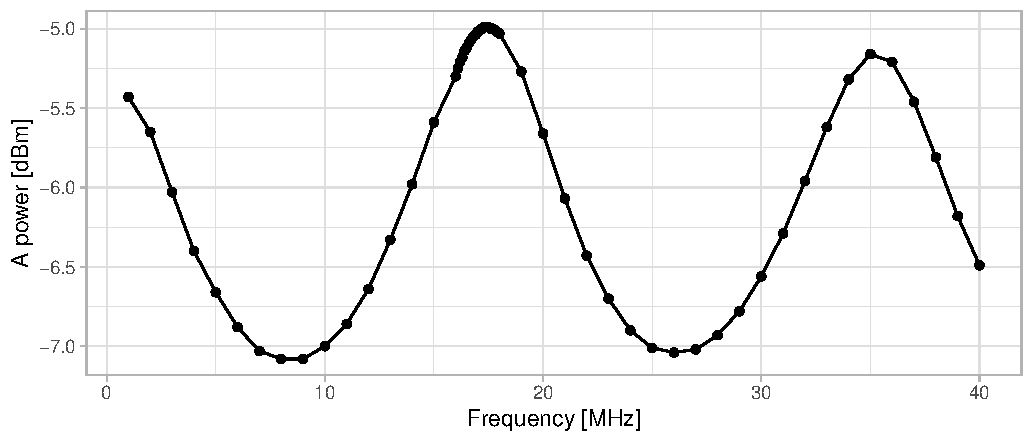
\includegraphics[width=\linewidth]{data/1_2/power_vs_freq.pdf}
  \caption{Aの信号電力の周波数依存性.}
  \label{fig:1_4}
\end{figure}


\begin{figure}[H]
  \centering
  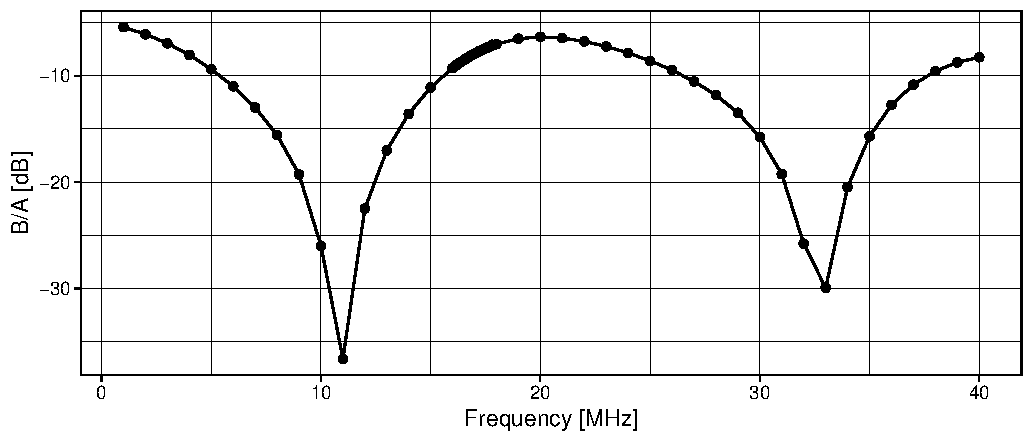
\includegraphics[width=\linewidth]{data/1_2/power_ratio_vs_freq.pdf}
  \caption{AとBの電力比の周波数依存性.}
  \label{fig:1_5}
\end{figure}

Aの信号電力には17.40 [MHz] 及びその約2倍の35 [MHz] の時にAの信号電力が最大となることが分かった.
また,AとBの電力比については,11 [MHz] 及び33 [MHz] のときに最小となることが分かった.
なお,Aの極大値を正確に測定するために,17 [MHz]付近は0.1 [MHz]刻みで測定を行った.


\subsubsection{考察}
まず始めに,同軸ケーブルによる信号の減衰について測定した結果を考察する.
高周波ほど,単位長さあたりの減衰率が大きくなることが分かった.
したがって,このことから高周波実験においてはケーブル長さをむやみに長くすることは,信号の減衰を生じさせてしまうため,注意が必要であることが分かった.

次に,信号の重ね合わせについて測定した結果を考察する.

まず始めに,AとBの電力比に周波数依存性が生じた理由について考える.
これは,Aの電力にも周波数依存性はあるものの,そのオーダーは高々1桁程度であるため,この周波数依存性はB端子に入力される信号の周波数依存性に起因するものと考えられる.
B端子に入力される信号は,1 [m] と10 [m] の同軸ケーブルを並列に接続しているため, これら2本の同軸ケーブル間には9 [m] 分の位相差が生じる.
先の実験から,同軸ケーブル中の光速度 (伝送速度) $v$は約$v = 2.0 \times 10^8$ [m/s] であることが分かっている.
$d = 9$ [m] での位相の変化は,
\begin{equation}
  \delta = \frac{2\pi}{\lambda}d
\end{equation}
であって,2つの信号が干渉によって弱めあう条件は,逆位相となればよいから,
\begin{equation}
  \delta = (2n + 1)\pi \quad (n = 0, 1, 2, \cdots)
\end{equation}
従って,これから,打ち消しあう周波数$f = \frac{v}{\lambda}$は,
\begin{equation}
  f = \frac{v}{\lambda} = v \frac{(2n + 1)}{2\pi d} \approx 11, 33, \cdots \mathrm{[MHz]}
\end{equation}
となり,確かに実験結果と一致していることが分かる.

次に,Aの信号電力に周波数依存性が見られた理由について考える.
このような周波数依存性はB端子に見られたように,何らかの信号との干渉によって生じたものであると考えられる.
そのような干渉を起こす信号との伝送距離の差を$d'$とすると,信号が強めあうためには同位相$\delta' = 2n\pi$である必要があることから同様にして求めると,
\begin{equation}
  d' = n\lambda = \frac{n v}{f}
\end{equation}
ここで,$f = 17.40$ [MHz] に最初の干渉が見られたことから,$d' = 11.5$ [m] 及びその整数倍であることが分かる.
テキスト図18のように回路を組んだことから,一度パワーディバイダでB端子側へ分割され1 [m] のケーブルと10 [m] のケーブルを介して再度パワーディバイダを通ってA端子へ伝送された信号が干渉である可能性が高いと考えられる.
$d'$が正確に11 [m] でなかった要因としては,同軸ケーブルどうしを繋ぐコネクタ等によるもので考えられる.
そこでコネクタの長さを測定すると,往路と復路合計で約0.45 [m]であり,確かに実験の結果と一致していることが分かる.

% \subsection{パワーメータによる測定}
% \subsubsection{方法}

% \subsubsection{結果}

% \subsubsection{考察}


\section{課題2: インピーダンス不整合による電磁波の反射}
\subsection{方法}
本実験では方向性結合器を用いて,インピーダンス不整合による電磁波の反射について測定を行った.
ここで,方向性結合器はIN--OUT間で信号をよく透過し,IN--FWD間ではわずかに信号を透過,FWD--OUT間では信号を透過しないような特性を持つ.

まず始めに,方向性結合器の特性を調べるために,テキスト図19のように回路を構成し,信号発生器で発生させた正弦波(10 [MHz], 10 [dBm])
を方向性結合器の入力端子を変えながら接続し,出力信号から方向性結合器の透過率および伝播時間を測定した.
ここで,方向性結合器の接続方法は次の表\ref{table:2-1}に示す通りである.
また,用いた方向性結合器はDC060であり,この方向性結合器はIN-FWD間で信号を反転させる特性を持つ.

\begin{table}[H]
    \centering
    \caption{方向性結合器の接続方法.}
    \label{table:2-1}
    \begin{tabular}{cccc}
        \hline
        & IN & OUT & FWD \\
        \hline\hline
        (1) & 透過出力信号 & 50\si{\ohm}終端 & 入力\\
        (2) & 入力 & 透過出力信号 & 50\si{\ohm}終端\\
        \hline
    \end{tabular}
\end{table}

次に,FWDを入力,OUTを出力とし,IN端子の終端条件を変えることで,インピーダンス不整合による反射率を測定した.
終端条件は次の表\ref{table:2-2}に示す通りである.
\begin{table}[H]
    \centering
    \caption{IN端子の終端条件.}
    \label{table:2-2}
    \begin{tabular}{cc}
        \hline
        & 終端条件\\
        \hline\hline
        (1) & 開放 ($Z_L = \infty$ [\si{\ohm}])\\
        (2) & 短絡 ($Z_L = 0$ [\si{\ohm}])\\
        (3) & 50\si{\ohm}終端 ($Z_L = 50$ [\si{\ohm}])\\
        (4) & 75\si{\ohm}終端 ($Z_L = 75$ [\si{\ohm}]) \\
        \hline
    \end{tabular}
\end{table}

さらに,IN終端条件をコイル ($L = 0.22$ [\si{\milli\henry}],)およびコンデンサ ($C = 100$ [\si{\pico\farad}])に変更し,インピーダンス不整合による反射率を測定した.
ただし,ここでは周波数を10, 20, 50, 100 [MHz]の4点で測定を行った.

\subsection{結果}
まず始めに,方向性結合器の特性について調べた結果について調べた結果を次の表\ref{table:2-3}に示す.
表\ref{table:2-1}に示した組み合わせにおいて,(1)では0.11の減衰と信号の反転が見られたが,(2)では信号の減衰や反転は見られなかった.
\begin{table}[H]
    \centering
    \caption{方向性結合器の特性.ここで表中の(1), (2)は表\ref{table:2-1}に示した接続方法に対応する.}
    \label{table:2-3}
    \begin{tabular}{cccc}
        \hline
        & 透過率 & 伝播時間 [\si{\nano\second}] & 位相差 [rad]\\
        \hline\hline
        (1) & 0.11 & 50.0& 3.14\\
        (2) & 1.0 & 0.00& 0.00\\
        \hline
    \end{tabular}
\end{table}

次に,IN端子の終端条件を変えたときの,インピーダンス不整合による反射率の測定結果を次の表\ref{table:2-4}に示す.
ただし,詳細は考察の節でも述べるが,先の測定からIN--FWD間で50 [ns] の時間差が生じることが分かっているため,時間差についてはIN-FWD間の時間差50 [ns]を引いて補正した値を示している.
\begin{table}[H]
    \centering
    \caption{IN端子の終端条件とインピーダンス不整合による反射率の測定結果.\\ここで,時間差についてはIN-FWD間の時間差を補正した値である.}
    \label{table:2-4}
    \begin{tabular}{cccc}
      \hline
      終端条件 & 反射率 & 時間差(補正値) [ns] & 位相差 [rad] \\
      \hline\hline
      開放        & 0.80   & -0.4                        & 0.0251          \\
      短絡       & 0.76   & -48.8                       & 3.07             \\
      50\si{\ohm}終端      & 0.012   & -50                         & 3.14             \\
      75\si{\ohm}終端      & 0.16   & 0.00                           & 0.00              \\     
      \hline
    \end{tabular} 
\end{table}

最後に,終端条件をコイルおよびコンデンサに変更して測定を行った結果を次の図\ref{fig:2-1}から図\ref{fig:2-4}に示す.
ただし,先の実験結果から,IN-FWD間で位相が逆位相になることに注意して,位相差は補正を行っている.
また,図\ref{fig:2-2}および図\ref{fig:2-4}では,式\eqref{eq:coil_phase}および式\eqref{eq:condenser_phase}より与えられる位相差の理論値をそれぞれ破線で重ねて示している.
\begin{figure}[H]
    \centering
    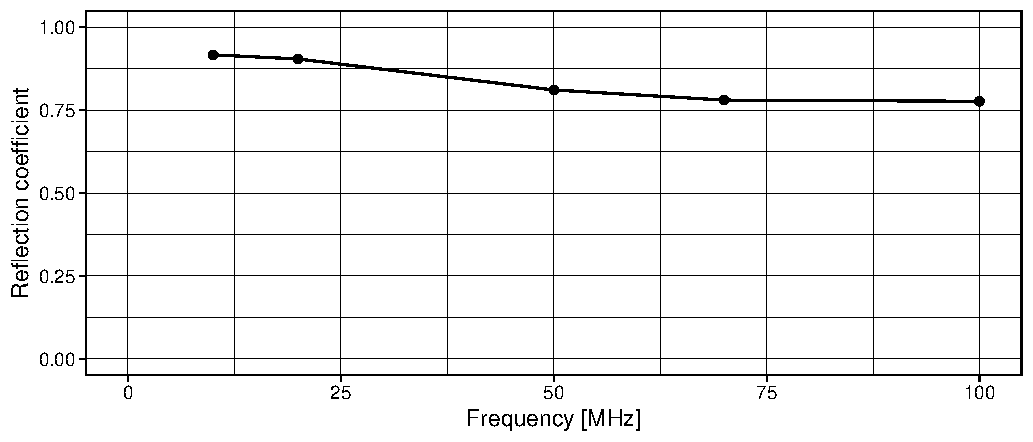
\includegraphics[width=\linewidth]{data/2_1/reflection_vs_freq.pdf}
    \caption{コイルのインピーダンス不整合による反射率の周波数依存性.}
    \label{fig:2-1}
\end{figure}

\begin{figure}[H]
  \centering
  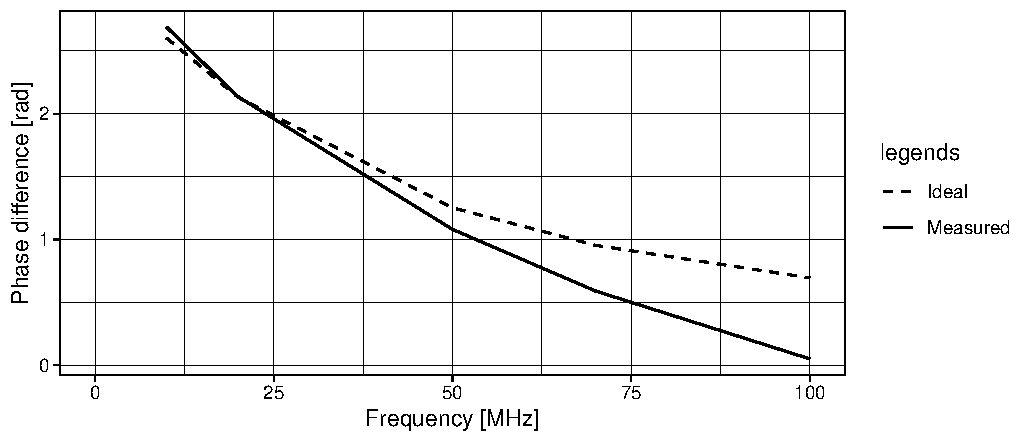
\includegraphics[width=\linewidth]{data/2_1/phase_diff.pdf}
  \caption{コイルのインピーダンス不整合による位相差の周波数依存性.}
  \label{fig:2-2}
\end{figure}

\begin{figure}[H]
  \centering
  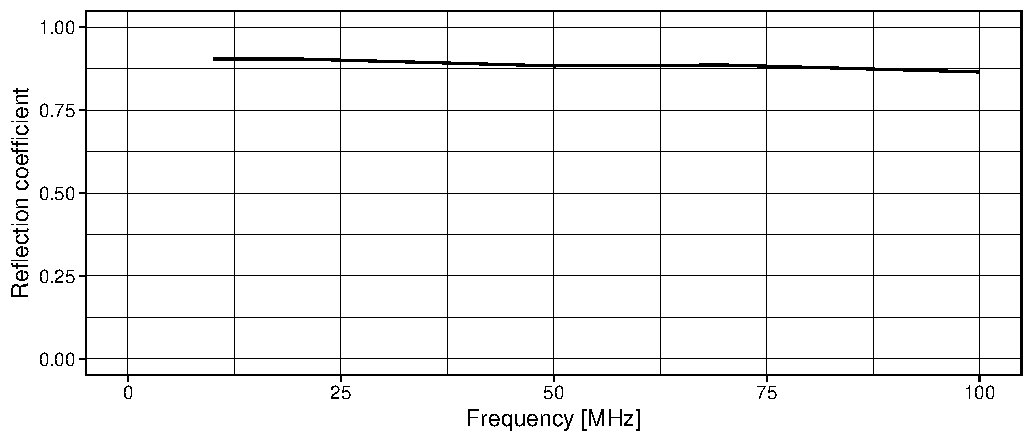
\includegraphics[width=\linewidth]{data/2_2/reflection_vs_freq.pdf}
  \caption{コンデンサのインピーダンス不整合による反射率の周波数依存性.}
  \label{fig:2-3}
\end{figure}

\begin{figure}[H]
\centering
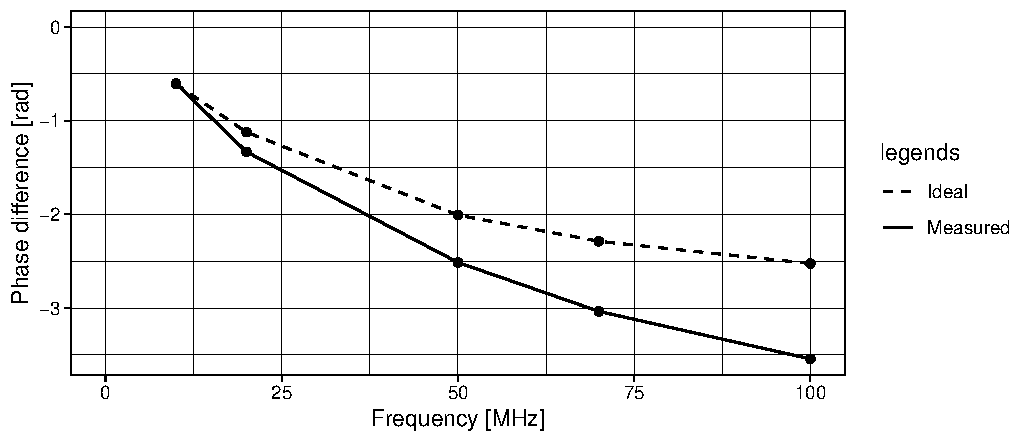
\includegraphics[width=\linewidth]{data/2_2/phase_diff.pdf}
\caption{コンデンサのインピーダンス不整合による位相差の周波数依存性.}
\label{fig:2-4}
\end{figure}

\subsection{考察}
まず始めに,方向性結合器の特性について調べた結果を考察する.
測定の結果から,終端は50 [\si{\ohm}]で整合しているため反射はないことと,方向性結合器はOUT-FWD間で直接には信号が伝わらないことに注意すると,IN-FWD間では信号が逆位相となって伝わることが分かる.
これは,テキストに述べられているような用いた方向性結合器DC060の特徴と合致する.

次に,インピーダンス不整合による反射率の測定結果について考察する.
開放・短絡時には反射率の大きさは1に近く,短絡時には逆位相となった.
また,整合時には反射率は限りなく低くなり,不整合の75\si{\ohm}終端時には反射率は僅かに大きいものの,位相差は0となった.
これは,原理の節の式\ref{eq:transmission}で述べたようなインピーダンスと反射率の関係と一致している.
50\si{\ohm}のときに位相が逆位相であったことから,実際には入力側のインピーダンスは50\si{\ohm}よりも僅かに大きい,
もしくは用いた50\si{\ohm}終端のインピーダンスが50 [\si{\ohm}] よりも僅かに小さいことが考えられる.

最後に終端条件をコイル・コンデンサに変更して測定した結果について考察する.
いずれの場合も反射率は1に近く,式\ref{eq:coil_phase}および式\ref{eq:condenser_phase}より与えられる反射率の絶対値が$|\Gamma| = 1$ことと一致している.
高周波領域で僅かに減少していることから,高周波領域で顕著に現れる残留抵抗や誘電損によるコンダクタンスの影響が考えられる.

また,位相差については,低周波領域では理論値と整合したものの特に高周波領域で乖離が見られた.
そこで,テキストp.143において,方向性結合器の透過率と伝播時間は周波数に依存しないと述べられているが,実際には周波数による変化がある可能性が考えられる.
そこで,FWD-IN間の伝播時間を周波数を変えて測定を行い,その結果から位相差にさらに補正を行った.
その結果を先の図\ref{fig:2-2}, \ref{fig:2-4}に重ねたものを,次の図\ref{fig:2-5}および図\ref{fig:2-6}に示す.
\begin{figure}[H]
    \centering
    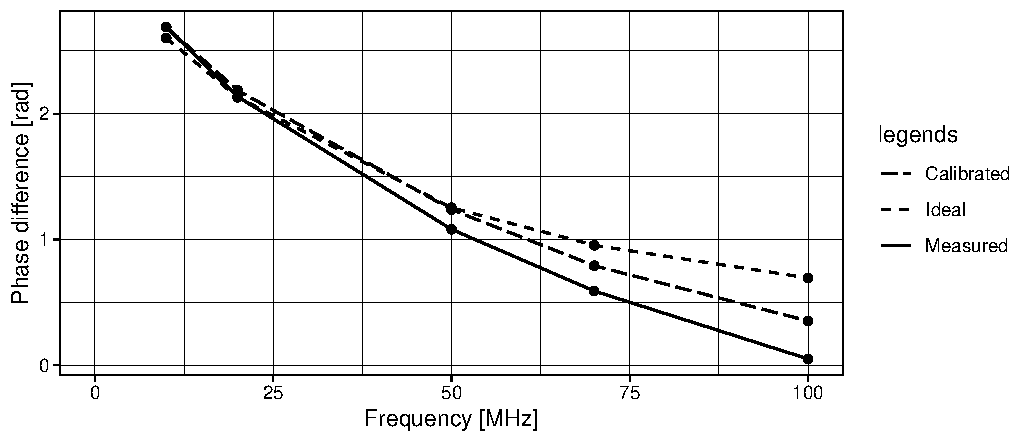
\includegraphics[width=\linewidth]{data/2_1/phase_diff2.pdf}
    \caption{コイルのインピーダンス不整合による位相差の周波数依存性.}
    \label{fig:2-5}
\end{figure}

\begin{figure}[H]
  \centering
  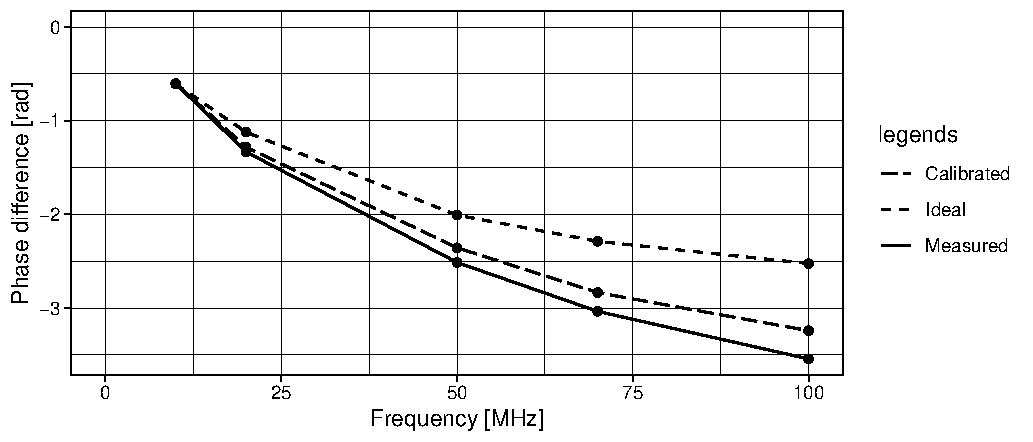
\includegraphics[width=\linewidth]{data/2_2/phase_diff2.pdf}
  \caption{コンデンサのインピーダンス不整合による位相差の周波数依存性.}
  \label{fig:2-6}
\end{figure}

高周波領域で理論値に近づいたものの,それでもなお高周波領域では乖離が見られた.
これらの原因としては,高周波領域で顕著になる浮遊容量や残留インダクタンスによるものが考えられる.

最後に,これら実験の結果を踏まえて,実験課題1において入力カップリングを1 \si{\mega \ohm}に設定した際に波形が乱れた原因について考察する.
これは,入力側のインピーダンスが50 \si{\ohm}であったのに対し,それよりも大きいインピーダンスを持つ負荷が接続されたことになるため,インピーダンス不整合が生じたことが原因であると考えられる.
このとき1 \si{\mega \ohm}は50 \si{\ohm}よりも十分大きいため,反射率は限りなく1に近いものと考えられ,これによって反射された信号がさらに不整合によって発生源である標準信号発生器やパワーメータのA端子側などと反射・干渉を起こし,結果として波形が乱れたものと考えられる.

\section{課題3: 集中定数回路と分布定数回路における共振特性}
\subsection{方法}
集中定数回路であるLC直列共振回路や分布定数回路であるオープンスタブ (試験体) を伝送経路に組み込み,それぞれの共振特性を測定した.
回路の構成としてはテキスト図21のように,6 [dB]のアッテネータを介して試験体へ信号を入力し,試験体から透過される信号を測定した.

LC直列共振回路の構成としては,$L = 0.22$ [\si{\micro \henry}]のコイルと$C = 3$ [\si{\pico \farad}]のコンデンサを用いた. 
また,オープンスタブとしてはマイクロストリップ線路を用いた.
各パラメタはテキスト図7に従うと,$\varepsilon_r = 4.4, h = 1.6\mathrm{\,[mm]}, w = 3\mathrm{\,[mm]}, t = 35\mathrm{\,[\mu m]}$である.
また,マイクロストリップ線路の長さは,根本から末端まで$d = 0.1791\mathrm{\,[m]}$である.

\subsection{結果}
LC直列共振回路の共振特性を測定した結果を次の図\ref{fig:3-1}に示す.
透過率が最小となったのは,周波数$f = 20.0$ [MHz] であり,このときの透過率は-5.29 [dB]であった.
\begin{figure}[H]
    \centering
    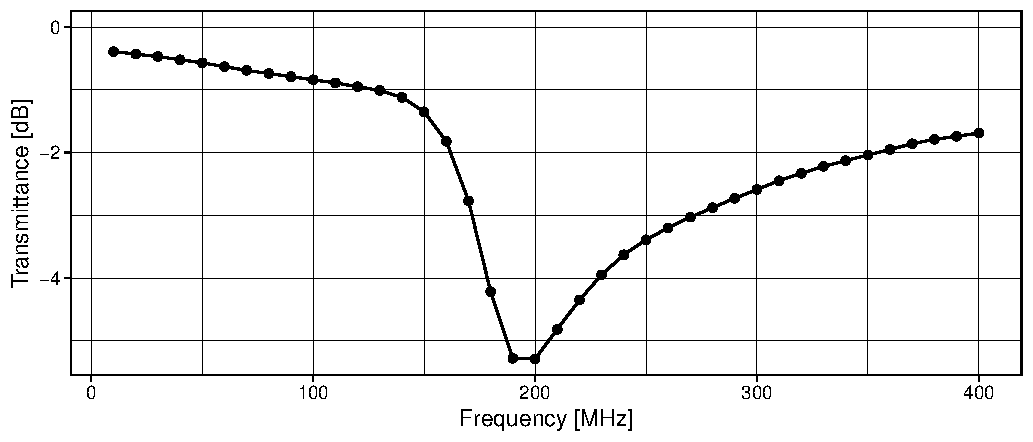
\includegraphics[width=\linewidth]{data/3_1/transmittance.pdf}
    \caption{LC直列共振回路の共振特性.}
    \label{fig:3-1}
\end{figure}

次に,オープンスタブの共振特性を測定した結果を次の図\ref{fig:3-2}に示す.
透過率が極小になったのは,周波数$f = 240, 733$ [MHz] であり,このときの透過率はそれぞれ-22.64, -13.71 [dB]であった
\begin{figure}[H]
    \centering
    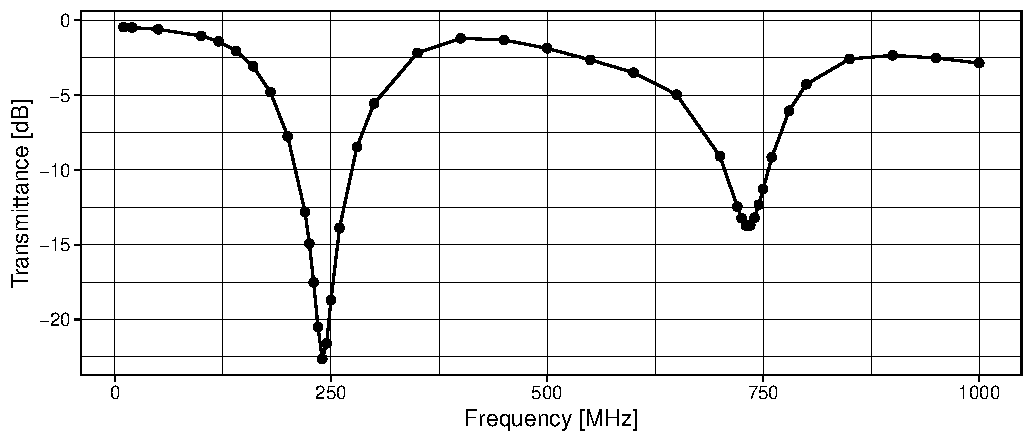
\includegraphics[width=\linewidth]{data/3_2/transmittance.pdf}
    \caption{オープンスタブの共振特性.}
    \label{fig:3-2}
\end{figure}


\subsection{考察}
まず始めに,LC直列共振回路の共振特性について考察する.
LC直列共振回路おいては,共鳴時に電力透過率が最小となった.
これは,共振回路の共鳴周波数$f$を求めると,式\eqref{eq:resonance_frequency}から$f = 196$ [MHz]であり,
このときLC直列回路のインピーダンスは0になる.
すなわち,伝送経路の途中にインピーダンスが0の回路が挿入されるため,式\eqref{eq:reflection_3}および式\eqref{eq:transmission}より,すべての信号が反射されるため透過率は0となる.


一方で,オープンスタブの共振周波数には周期性が見られた.
マイクロストリップ線路の設計から特性インピーダンスと伝送速度を求めると,$Z_L = 50$ [\si{\ohm}],$v = 1.66\times 10^8$ [m/s]であることが分かる.
このとき,式\eqref{eq:resonance_length}に示したように,回路の共鳴条件は末端を固定端,根本を自由端としたときの共鳴条件と合致し,
共鳴周波数を求めると,最小の周波数から順に$231, 693, \dots$ [MHz]であることが分かる.
観測された周波数との誤差はそれぞれ3.7, 5.3 [\%]であり,
マイクロストリップ線路の設計値には誤差が含まれていることも考慮すると,十分に一致していることが分かる.
また,このように周期的に共鳴するのは,先の述べたように気柱や弦のような固定端--自由端の共鳴条件に起因するものであると考えられる.
すなわち,電圧を印加している端子は末端が解放されているため,電流は常に0の固定端としてふるまう一方で,根本側は交流電源によって電流が時間変動する自由端に相当する.
そのため,このような共鳴条件が生じると考えられる.

\section{課題4: ヘテロダイン検波}
\subsection{方法}
テキスト図22のように,DBMを用いてファンクションジェネレータで生成した正弦波(10 [MHz], 0 [dBm])と,
標準信号発生器で発生させた局所信号(正弦波, 0 [dBm])を混合させ,オシロスコープに表示される波形を観測した.

さらに,特性周波数$f_c$を$f_c = 1$ [MHz]とし,2 [MHz]における減衰量が15 [dB]以上となるようにローパスフィルタ(LPF)を作成し,
テキスト図23のように標準信号発生器からの信号を入力してその特性を確認した.
ここで,LPFの設計についてはテキスト図29のような構成に従い,設計条件から$n = 3$とした.
設計したLPF回路の概略を図\ref{fig:4-circuit}に示す.
\begin{figure}[H]
    \centering
    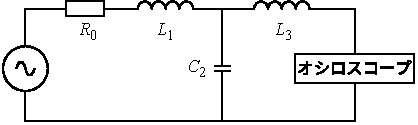
\includegraphics[width=0.7\linewidth]{img/LPF.pdf}
    \caption{ローパスフィルタ回路の概略.}
    \label{fig:4-circuit}
\end{figure}
このとき,$f = 2$ [MHz]における減衰量は$1/(1 + (f/f_c))^{2n} = 0.015 = 18$ [dB]となる.
また,各素子については,$L_1  = 8.0$ [\si{\micro \henry}],$C_2 = 6.4$ [\si{\nano \farad}],$L_3 = 8.0$ [\si{\micro \henry}]であるが,用いた素子の都合から,実際には
$L_1  = 7.92$ [\si{\micro \henry}],$C_2 = 6.170$ [\si{\nano \farad}],$L_3 = 7.80$ [\si{\micro \henry}]
である.

このLPFを用いてDBMで混合した信号から低周波成分を取り出し,そのときの波形の信号振幅と周波数を確認した.

\subsection{結果}
結果を図\ref{fig:4-1}に示す.
標準信号発生器から発生させた局所信号の周波数が,ファンクションジェネレータで発生させた信号の周波数10 [MHz]と一致しているときには整った波形がみられ,
一致しないときにはうなりを伴った波形が観測された.
このとき発生したうなりは,9 [MHz]および11 [MHz]のとき両方で,ファンクションジェネレータの周波数と局所信号の周波数の差に等しい約1 [MHz]であった.
\begin{figure}[H]
    \centering
    \begin{minipage}
        [b]{0.45\linewidth}
        \centering
        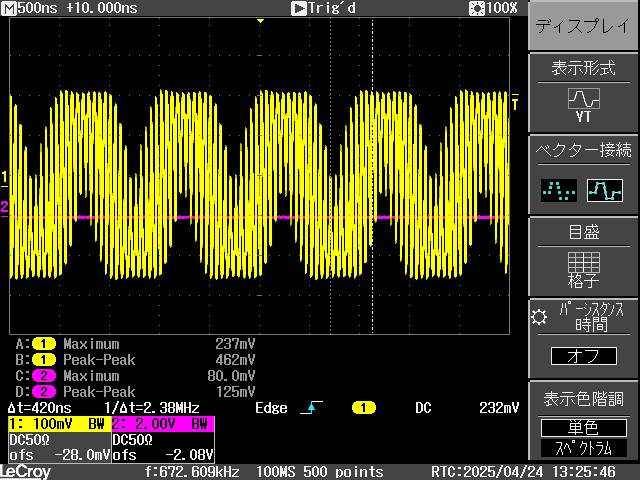
\includegraphics[width=\linewidth]{img/4_1_8MHz.jpg}
        \subcaption{9 [MHz]時.}
        \label{fig:4-1-a}
    \end{minipage}
    \begin{minipage}
        [b]{0.45\linewidth}
        \centering
        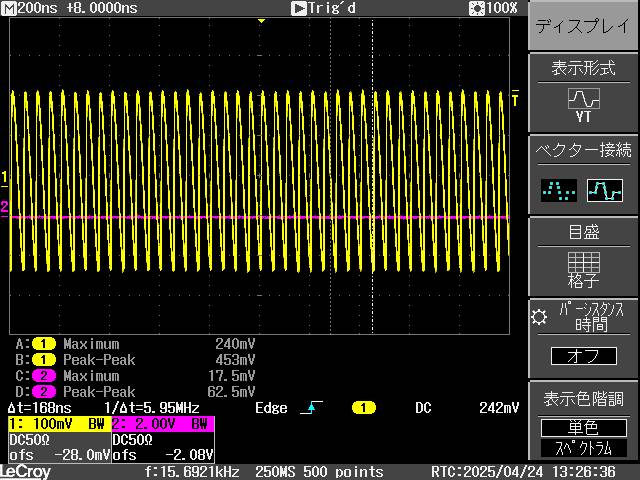
\includegraphics[width=\linewidth]{img/4_1_10MHz.jpg}
        \subcaption{10 [MHz]時.}
        \label{fig:4-1-b}
    \end{minipage}
    \begin{minipage}
        [b]{0.45\linewidth}
        \centering
        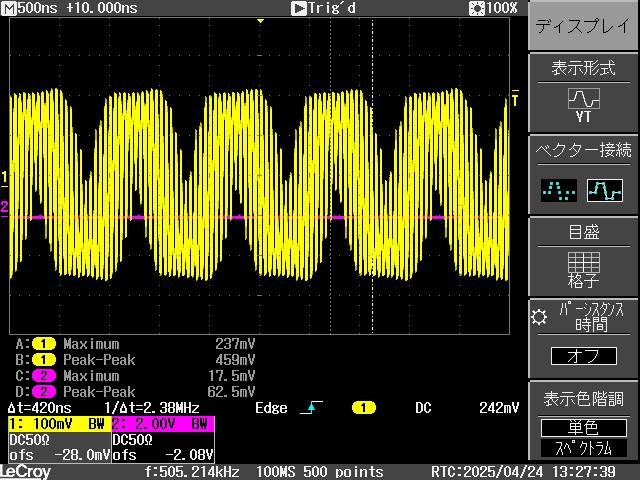
\includegraphics[width=\linewidth]{img/4_1_11MHz.jpg}
        \subcaption{11 [MHz]時.}
        \label{fig:4-1-c}
    \end{minipage}
    \caption{局所信号の周波数とオシロスコープで観察された信号波形.}
    \label{fig:4-1}
\end{figure}



次に,製作したLPFの周波数特性を測定した結果を図\ref{fig:4-2}に示す.
おおよそ設計値に一致していることが分かる.
\begin{figure}[H]
    \centering
    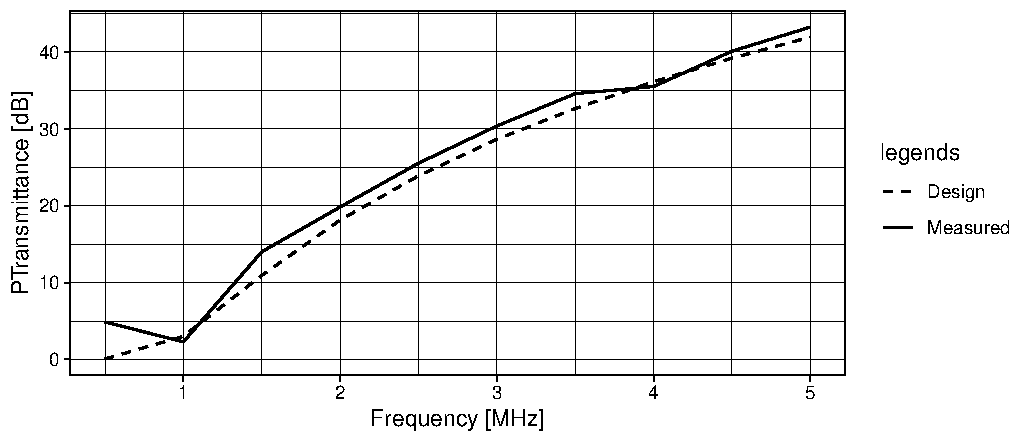
\includegraphics[width=\linewidth]{data/4_1/transmittance.pdf}
    \caption{LPFの周波数特性.実線が測定値,破線が設計値.}
    \label{fig:4-2}
\end{figure}

また,設計したローパスフィルタを用いて,DBMで混合した信号から低周波成分を取り出した結果を図\ref{fig:4-3}に示す.
局所信号の周波数の周波数が9 [MHz]および 11 [MHz]のときには,ファンクションジェネレータの周波数の差 1 [MHz]の信号が観測された.
また,局所信号とファンクションジェネレータの周波数が一致しているときには,信号はほとんど観測されなかった.
\begin{figure}[H]
  \centering
  \begin{minipage}
      [b]{0.45\linewidth}
      \centering
      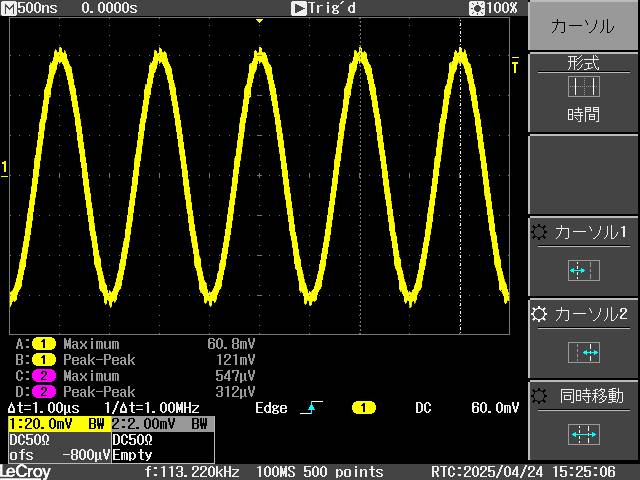
\includegraphics[width=\linewidth]{img/4_3_9MHz.jpg}
      \subcaption{9 [MHz]時.}
      \label{fig:4-3-a}
  \end{minipage}
  \begin{minipage}
      [b]{0.45\linewidth}
      \centering
      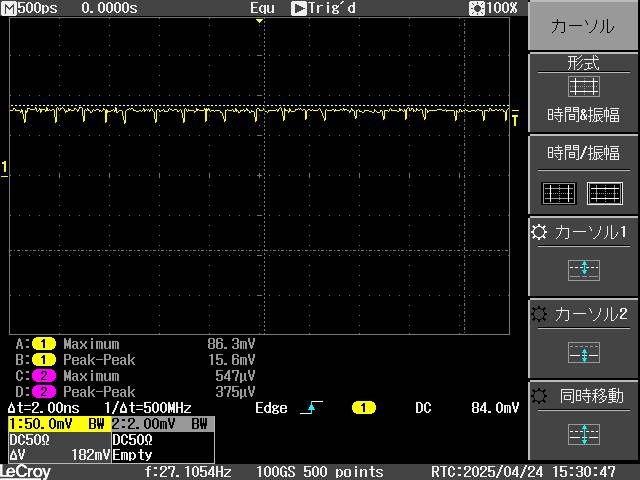
\includegraphics[width=\linewidth]{img/4_3_10MHz.jpg}
      \subcaption{10 [MHz]時.}
      \label{fig:4-3-b}
  \end{minipage}
  \begin{minipage}
      [b]{0.45\linewidth}
      \centering
      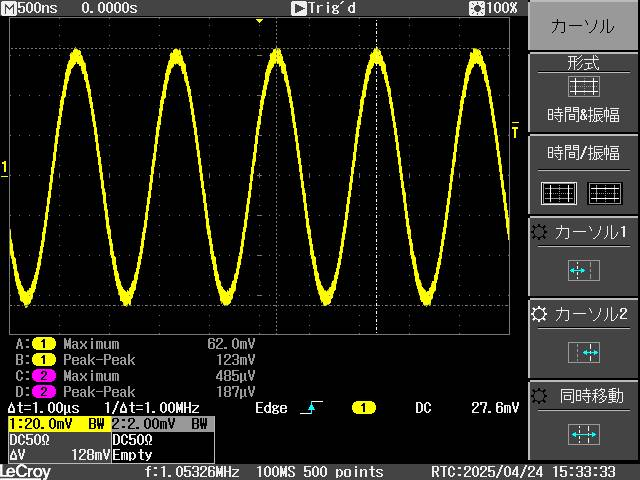
\includegraphics[width=\linewidth]{img/4_3_11MHz.jpg}
      \subcaption{11 [MHz]時.}
      \label{fig:4-3-c}
  \end{minipage}
  \caption{局所信号の周波数とLPFを介してオシロスコープで観察された信号波形.}
  \label{fig:4-3}
\end{figure}

\subsection{考察}
まずはじめにLPFのはたらきについて,コイル・コンデンサの周波数特性から定性的に確認する.
コイル,コンデンサのインピーダンスはそれぞれ$Z_L = i\omega L$,$Z_C = 1/(i\omega C)$である.
したがって,$f \to 0$つまり$\omega \to 0$のときにはコイルは短絡 ($Z_L \to 0$),コンデンサは開放 ($Z_C \to \infty$)となる.
一方で,$f \to \infty$つまり$\omega \to \infty$のときにはコイルは開放 ($Z_L \to \infty$),コンデンサは短絡 ($Z_C \to 0$)となる.
以上の考察を踏まえ,このときの回路の様子を模式的に表したものが,次の図\ref{fig:4-4}である.
図からも明らかなように,$f \to 0$のときには反射なく信号が透過し,逆に$f \to \infty$のときには信号が透過されないことが分かる.
以上のことから,定性的にLPFのはたらきを確認することができた.
\begin{figure}[H]
    \centering
    \begin{minipage}[b]{0.7\linewidth}
        \centering
        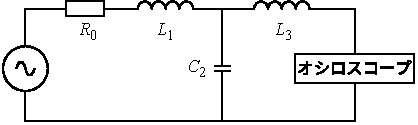
\includegraphics[width=\linewidth]{img/LPF.pdf}
        \subcaption{LPFの構成.}
        \label{fig:4-4-a}      
    \end{minipage}
    \begin{minipage}[b]{0.7\linewidth}
        \centering
        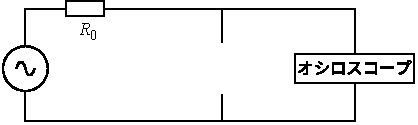
\includegraphics[width=\linewidth]{img/LPF_f_0.pdf}
        \subcaption{$f\to 0$のとき.}
        \label{fig:4-4-b}      
    \end{minipage}
    \begin{minipage}[b]{0.7\linewidth}
        \centering
        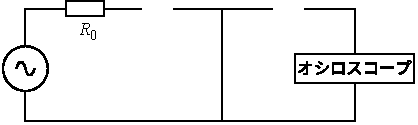
\includegraphics[width=\linewidth]{img/LPF_f_inf.pdf}
        \subcaption{$f\to \infty$のとき.}
        \label{fig:4-4-c}      
    \end{minipage}
    \caption{LPFの構成と周波数が0および無限大のときの回路の模式図.}
    \label{fig:4-4}
\end{figure}

また次に,ヘテロダイン検波が多くの情報通信や高周波物性測定に用いられる理由について考察する.

可視光やX線の観測,あるいや光通信においては,観測する対象は非常に高い周波数となる.
しかし,このような高周波を直接観測するのは難しく,また高周波ほど減衰などの影響を受けやすくなるため,受信側で情報を処理をする際には低周波であることが望ましいと考えられる.
このようなとき,ヘテロダイン検波を用い,予め周波数の分かっている局所信号と受信した信号を混合させ,そのうなりを観測することで,比較的容易に受信した信号の光を測定することができる.
ヘテロダイン検波による観測の長所としては,局所信号から大きく離れた信号は受信できないためノイズの影響を受けにくいこと,
局所信号の強度を高めることで微弱な信号でも受信できることが挙げられる\cite{heterodyne}.
一方で,観測対象の周波数が未知の場合や広範である場合には,ヘテロダイン検波の原理上,その周波数を同定することは難しいと考えられる.
しかし,多くの場合において観測対象の周波数は分かってることが多いため,このことが
ヘテロダイン検波が多くの情報通信や高周波物性測定によく用いられる理由であると考えられる.

% そこで,受信した信号をヘテロダイン検波を用いて位相情報や振幅の情報を保存したまま低周波 (中間波)に変換することで,
% 減衰などの影響を受けることなく処理することができると考えられる.
% これが,ヘテロダイン検波が多くの情報通信や高周波物性測定に用いられる理由であると考えられる.



\section{課題5: 半波長アンテナにおける電気双極子放射}
\subsection{方法}
テキスト図24のように,半波長アンテナを適当な距離$r$を介して設置し,標準信号発生器から発生させた正弦波(10 [dBm])を入力させた.
このとき,アンテナの放射強度比 (AとBの電力比) を種々の条件のもとに測定した.
ここで半波長アンテナの長さ$L$は0.201 [m]である.

まず始めに,アンテナの間隔を5 [cm]として机上に垂直かつ互いに平行になるようにおき,アンテナに印加する信号の周波数を変化さて受信側アンテナで測定される信号電力を測定することで,放射強度比を求めた.
このとき,放射強度が最大となる周波数$f_0$を求めた.
以降の測定では,この周波数のもとに測定を行った.
次にアンテナの間隔$r$を変化させて,放射強度比の距離依存性を測定した.
また,適当な距離$r$を介してアンテナを設置し,発信用アンテナを2アンテナが張る面内で回転させ,その回転角$\theta$と放射強度比との関係を測定した.
ここで,$\theta$は机上に対して垂直なときを$\theta = 90$ [deg]とする.
さらに,アンテナ同士が平行な状態から,発信用アンテナを受信用アンテナの方向を回転軸に水平に傾け,2アンテナが直交している場合の放射強度比の変化を測定した.
最後に,アンテナ同士を平行,5 [cm] 間隔に配置し,その隙間に厚紙,アクリル板,アルミ板を挿入したときの放射強度比の変化を測定した.


\subsection{結果}
アンテナに印加する信号の周波数を変えて受信強度を測定した結果を,次の図\ref{fig:5-1}に示す.
最大となったのは周波数$f_0 = 670$ [MHz]であり,このときの受信強度は8.9[dBm]であった.
\begin{figure}[H]
    \centering
    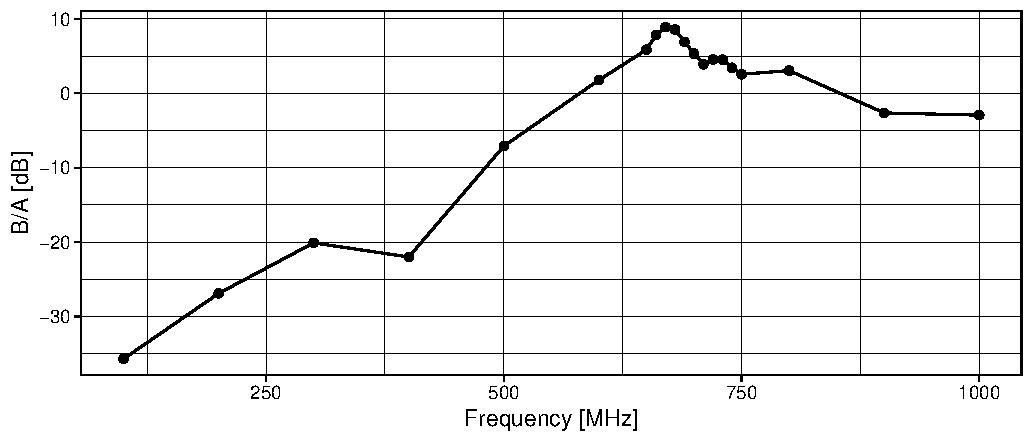
\includegraphics[width=\linewidth]{data/5_1/gain.pdf}
    \caption{印加する交流電源の周波数と放射強度の関係.}
    \label{fig:5-1}
\end{figure}

次に,アンテナ間の距離$r$を変化させて放射強度比の距離依存性を測定した結果を次の図\ref{fig:5-2}に示す.
\begin{figure}[H]
  \centering
  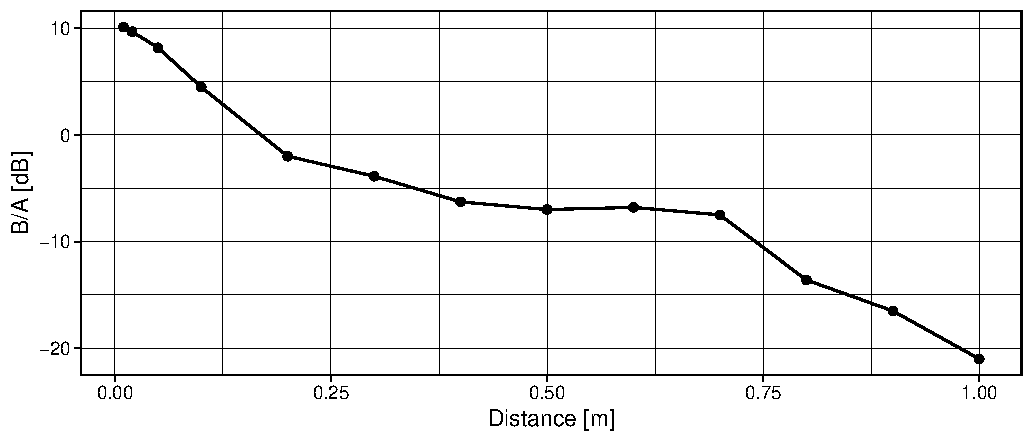
\includegraphics[width=\linewidth]{data/5_2/gain.pdf}
  \caption{アンテナ間の距離$r$と放射強度の関係.}
  \label{fig:5-2}
\end{figure}
十分離れた点では式\eqref{eq:power_received}から$P \propto r ^ {-2}$であるから,$10\log_{10} P \propto -20 \log_{10} r$となり,
放射強度の単位をdBで表したとき,距離を対数スケールで表すと傾きが-20の直線となることが予想される.
そこで,距離が0.1 [m] よりも遠い場合について,片対数グラフで示したのが次の図\ref{fig:5-3}である.
\begin{figure}[H]
    \centering
    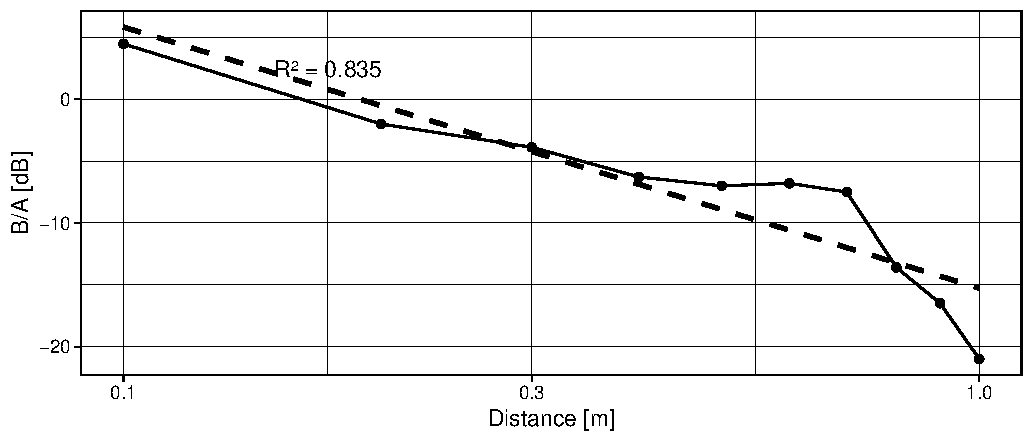
\includegraphics[width=\linewidth]{data/5_2/gain2.pdf}
    \caption{アンテナ間の距離$r$と放射強度の関係.ただし,$r> 0.1$ [m]について示している.}
    \label{fig:5-3}
\end{figure}
また,最小二乗法によって傾きを求めると,$-21$であった.

次に,回転角$\theta$を変えたときの放射強度比との関係を測定した結果を次の図\ref{fig:5-4}に示す.
ここでアンテナの距離は0.3 [m] とした.
\begin{figure}[H]
    \centering
    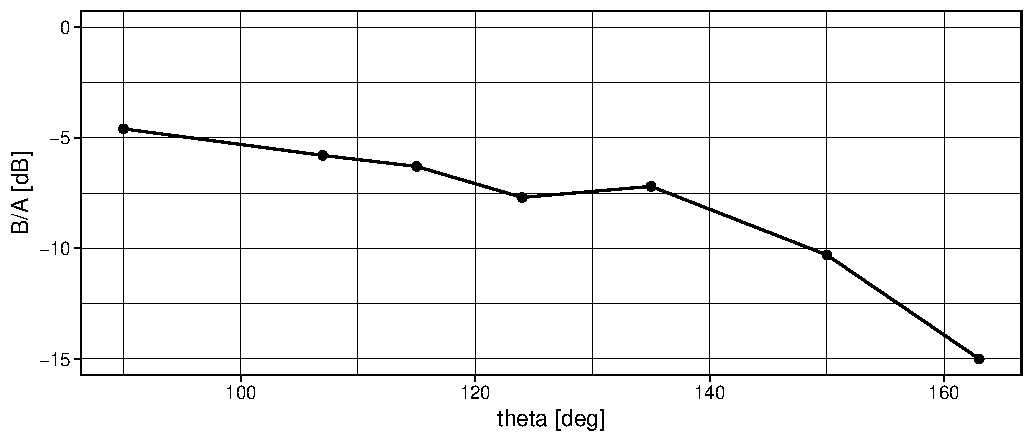
\includegraphics[width=\linewidth]{data/5_3/gain.pdf}
    \caption{回転角$\theta$と放射強度の関係.}
    \label{fig:5-4}
\end{figure}
十分離れた点では $P \propto \sin^2 \theta$ であるから,$10\log_{10} P \propto 20 \log_{10} \sin \theta$となり,
同様に放射強度の単位をdBとし,角度の正弦を対数スケールでプロットすると傾き20の直線となることが分かる.
そこで,片対数グラフで示したのが次の図\ref{fig:5-5}である.
\begin{figure}[H]
    \centering
    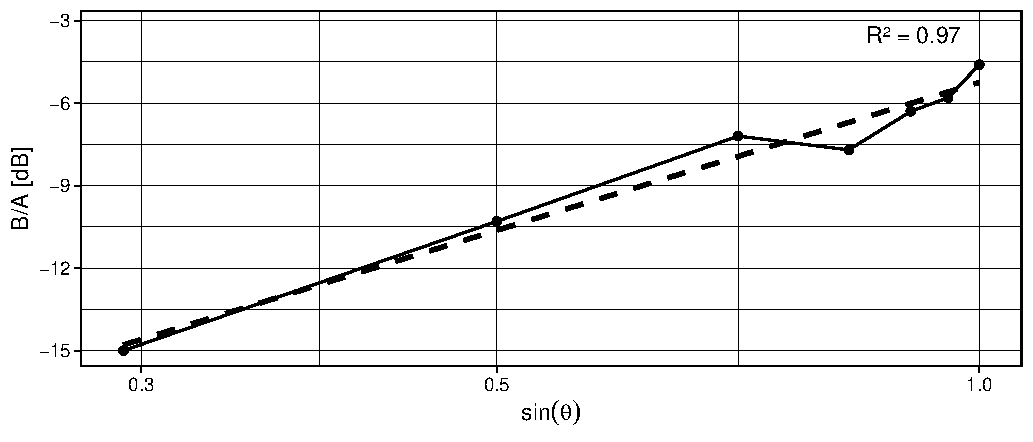
\includegraphics[width=\linewidth]{data/5_3/gain2.pdf}
    \caption{回転角$\theta$の正弦と放射強度の関係.}
    \label{fig:5-5}
\end{figure}
また,最小二乗法で傾きを求めると,18であった.

次に,アンテナを直交させたときの放射強度比について測定した結果を次の表\ref{table:5-1}に示す.
アンテナを直交させることで,平行時には0.10 [dB]であったアンテナの放射強度比は-8.7 [dB]となった.
なお,このときのアンテナ間の距離は0.3 [m]である.
\begin{table}[H]
    \centering
    \caption{2アンテナを平行・直交にしたときの放射強度比.}
    \label{table:5-1}
    \begin{tabular}{cc}
        \hline
        & 放射強度比 [dB]\\
        \hline
        \hline
        平行 & 0.10\\
        直交 & -8.7\\
        \hline
    \end{tabular}
\end{table}

最後に,アンテナ間に物体を挿入したときの放射強度比について測定した結果を次の表\ref{table:5-2}に示す.

\begin{table}[H]
    \centering
    \caption{アンテナ間に物体を挿入したときの放射強度比.}
    \label{table:5-2}
    \begin{tabular}{ccc}
        \hline
        & 放射強度比 [dB] & 減衰率 [dB]\\
        \hline
        \hline
        無 & 8.2 & 0 \\
        厚紙 & 7.8 & 0.4\\
        アクリル板 & 7.63 & 0.57\\
        アルミ板 & -21.2 & 29.4\\
        \hline
    \end{tabular}
\end{table}


\subsection{考察}
まず始めに,アンテナ長さと$f_0$における半波長との関係について述べる.
$f_0 = 670$ [MHz]のとき,半波長の長さは$\lambda / 2 = 0.223$ [m]であり,半波長アンテナ長さ$L = 0.201$ [m]と非常に近いことが分かる.
これは,先の実験4のときのオープンスタブと同様に,
アンテナ中央を自由端,両端を固定端として,アンテナ上で共鳴が生じているためであると考えられる.
% すなわち,アンテナは開放されていることから,インピーダンスは無限大であり,
% 理論的には反射率は1となるため,式\eqref{eq:resonance_length}と同様の共鳴条件が成立する.
% そのため,半波長とアンテナ長さが一致したときに,共鳴によって放射強度が最大となったと考えられる.
ここで,半波長アンテナの長さよりも半波長の長さが長いのは,机などからの反射によって実効的な長さが長くなっているためであると考えられる.

次に,式\eqref{eq:power_received}に示した関係が成り立つことを確認する.
これは,図\ref{fig:5-3}および図\ref{fig:5-5}に示したように,
強度 [dB] を縦軸にとり,距離や角度の正弦を横軸に片対数グラフで示すと傾きがそれぞれ-20, 20に近いことから,
先述べたように放射強度は距離の2乗に反比例し,角度の正弦の二乗に比例することが分かる.
したがって,十分離れた点では式\eqref{eq:power_received}が成り立つことが分かる.

さらに,アンテナ同士が直交したときに信号強度が減少する理由について考察する.
これは,アンテナが発生・受信する電磁波の偏波方向が直交することで,受信側で受信する信号が減少するためであると考えられる.
2つのアンテナのなす角を$\varphi$とすると,アンテナが送受信する電磁場の偏波方向のなす角もそれぞれ$\varphi$となる.
受信側アンテナでは自身の偏波方向の成分だけを受信するため,受信できる電磁波は$E, B \propto \cos \varphi$となり,強度は$P \propto E B \propto \cos^2 \varphi$となる.
すなわち,直交時 ($\varphi = \pi/2$ [rad]) には受信強度が0となることが予想されるが,測定時に完全に0にならなかった要因としては,机などの周囲からの反射によるものであると考えられる.

最後にアンテナ間に物体を挿入したときの放射強度比について考察する.
金属板を挿入したときに大きく信号が減衰したのは,媒質中を伝播する電磁波は指数関数的に減衰することに起因するものであると考えられる.
ここで,電磁波が媒質に侵入できる深さは式\eqref{eq:skin_depth}で与えられ,抵抗率が小さいほど浅くなる.
理科年表2025年度版から,アルミニウムの抵抗率は$\rho_{\ce{Al}} = 2.5 \times 10^{-8}$ [\si{\ohm \meter}]であるから,
これをもとにその深さを計算すると$\delta = 3$ [\si{\micro \meter}]である.
用いたアルミ板はこれよりも十分に厚いことから,電磁波はほとんど透過できないことが分かる.
また,この深さは抵抗率の平方根に比例することから,絶縁体の厚紙やアクリル板では,ほとんど減衰せずに透過することが分かる.

\section{結論}
% 実験目的を要約して記述し、それに対応する結論を簡潔に記述すること。

本実験では,まず始めに高周波測定を行う際の基礎を確認し,高周波では同軸ケーブルの減衰が顕著であることから
接続するケーブル長をむやみに長くすることは避けるべきであることを確認した.
その上で,基本的な性質としてインピーダンス整合・不整合時に電磁波の反射が見られるのか測定を行った.
その結果,インピーダンスが整合する際には反射が起こらず,不整合時に反射が見られること,コイル・コンデンサを終端に接続した際にはインピーダンスの周波数依存性に依る反射率の周波数依存性が確かめられた.
次に,直列LC共振回路とオープンスタブの共振特性を測定し,LC回路においてはコイルとコンデンサのインピーダンスの大きさが等しいときに共鳴が起き,
オープンスタブにおいて線路上に固定端--自由端の共鳴条件が成立するときに共鳴が生じることが分かった.
さらに,ヘテロダイン検波においては,DBMによって混合された波を,ローパスフィルタを用いることで低周波成分 (中間波) を取り出せることを確認した.
また,半波長アンテナを用いた実験では,アンテナの距離・周波数依存性が理論値と十分近いことが分かった.
また,半波長アンテナにおいてもオープンスタブと同様の共鳴条件により放射強度が最大化されることが分かった.

% 参考にした文献があれば記述する。以下の例を書き換えること。
\begin{thebibliography}{9}
  \bibitem{ref1}
    砂川重信. 電磁気学, 物理テキストシリーズ4. 岩波書店, 1977.

  \bibitem{heterodyne}
  森田隆二. 基礎講座 ホモダイン,ヘテロダインとは?. 応用物理, Vol.79, No.5. 2010.
    % \bibitem{bunken1}
    %     A. Einstein, B. Podolsky, and N. Rosen, 
    %     Phys. Rev. \textbf{47}, (1935) 777.
    %     % いわゆるEPRパラドックスと呼ばれる量子力学に関する論文

    % \bibitem{bunnken2}
    %     J.J. Aubert \textit{et al.},
    %     Phys. Lett. B \textbf{123} (1983) 275.
    %     % いわゆるEMC効果と呼ばれる現象についての実験の論文
    
\end{thebibliography}

\end{document}
